\section{Programos sudarymas ir rezultatai}

Pagal dviejų dimensijų skaitinį modelį \eqref{numerical-eqs} sudarytas uždavinį sprendžiantis skriptas ir kiti pagalbiniai skriptai duomenims vaizduoti ir tikrinti. Skriptai rašomi \textit{Python} programavimo kalba, naudojant \textit{NumPy}, \textit{SciPy}, \textit{Matplotlib} paketus. 

Modelio rezultatai yra saugomi kaip atskiri \textit{.npy} formato failai, kurie yra skirti saugoti \mbox{\textit{NumPy}} masyvus. Dėl praktinių rezultatų panaudojimo ir tyrimo nebūtina saugoti informacijos apie visus laiko žingsnius, todėl išsaugotuose rezultatų failuose, simuliacijos kadrai laiko kryptimi gali būti praretinti iki tūkstančio kartų, priklausomai nuo pasirinktų parametrų. Pagalbiniai duomenų vaizdavimo skriptai šiuos duomenis agreguoja į grafikus, kurie išsaugomi \textit{.png} formatu.

\begin{figure}[h!]
\centering
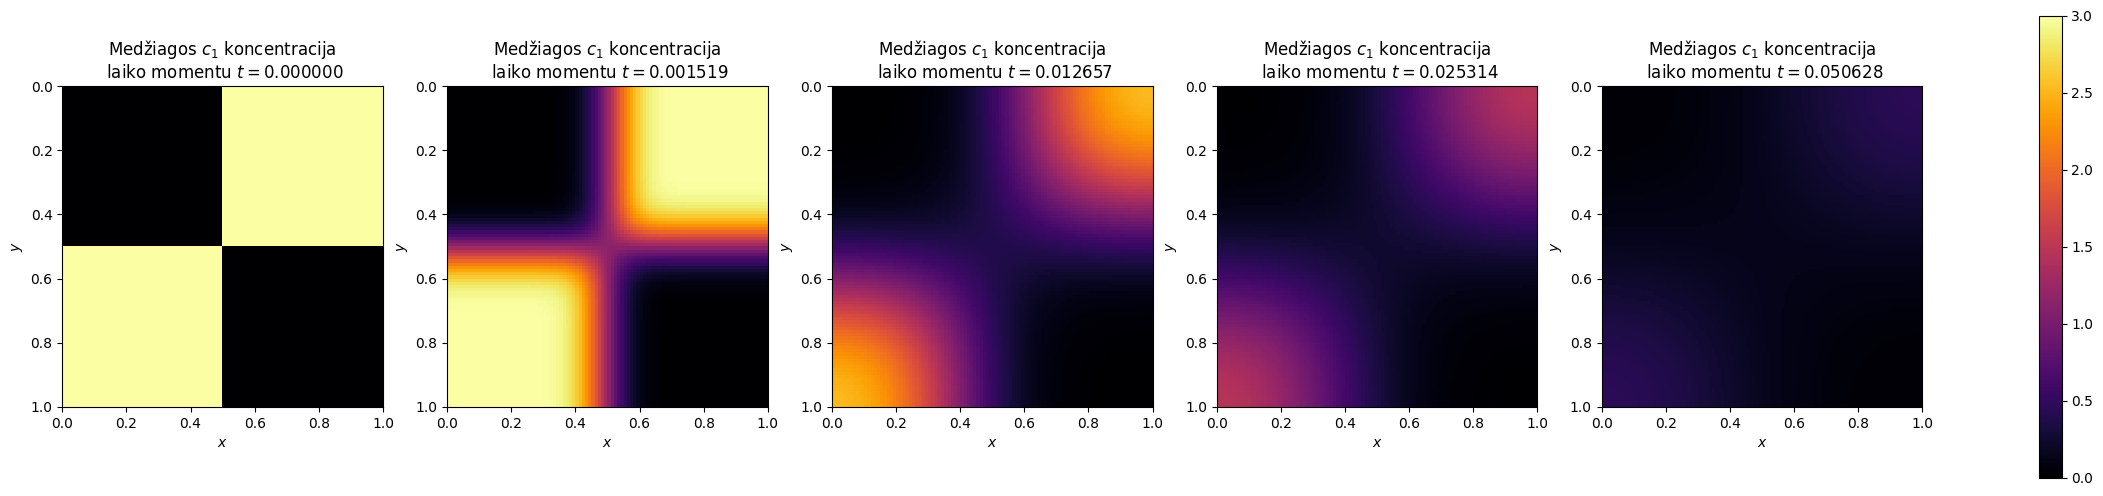
\includegraphics[width=\textwidth]{../assets/examples-c1.png} \\
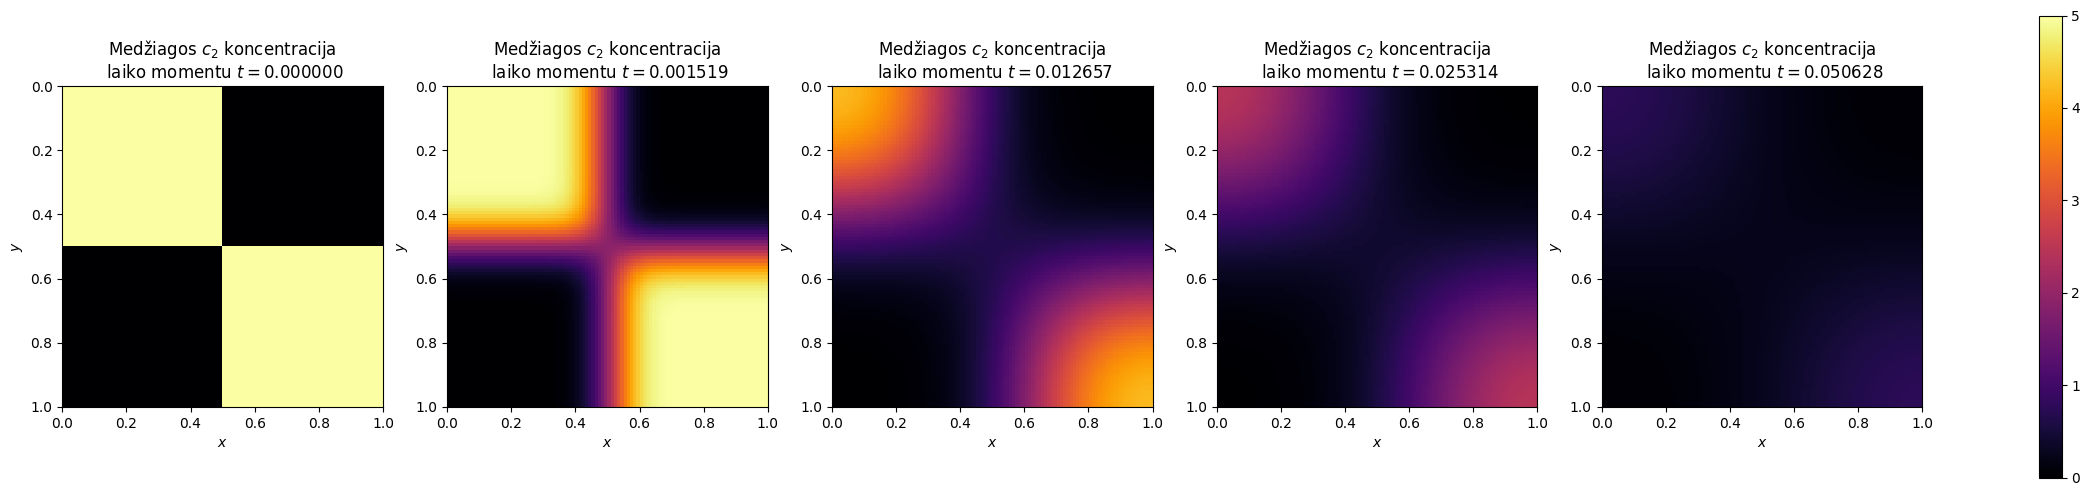
\includegraphics[width=\textwidth]{../assets/examples-c2.png} \\
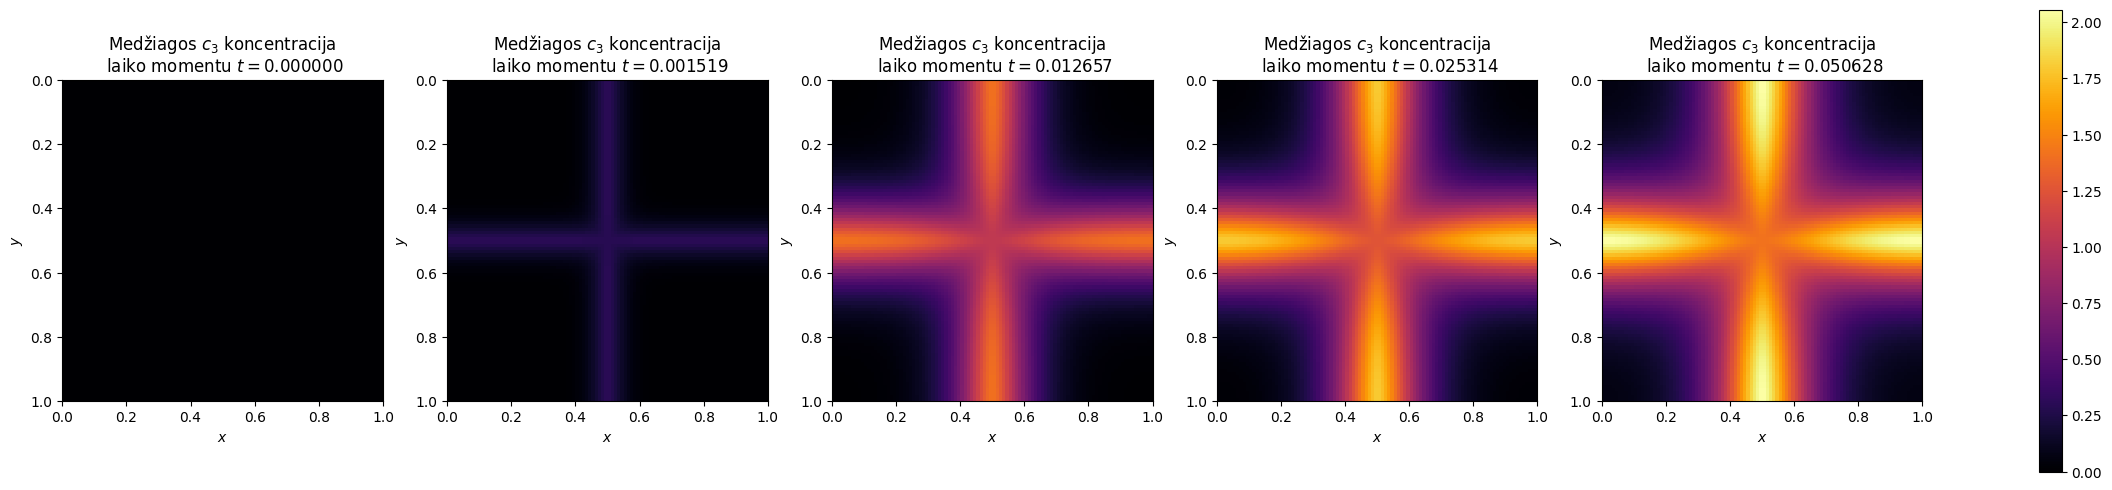
\includegraphics[width=\textwidth]{../assets/examples-c3.png}
\caption{Kompiuterinio modelio rezultato pavyzdys. $D = 0.05$, $W = 1$, $H = 1$, $\Delta x = \frac{1}{99}$, $\Delta y = \frac{1}{99}$, $k = 1$, $c_0 = 1$, $\Delta t$ - pasirinktas pagal \eqref{numerical-stability-condition} }
\label{result-example}
\end{figure}

\newpage
\subsection{Programos korektiškumo tikrinimas}

% Čia galima tikrint kad individualiu ląstelių
% - keičiant dx/dy kiekio per laiką sprendinys vizualiai konverguoja
% - kiekio grafikai per laika medžiagom c1 ir c2 mažėja, o c3 - didėja.
% - jei nustatom reakcijos koeficienta k = 0, kiekis bus pastovus
% Tikrinti rezultatų korektiškumui yra naudojami tie patys duomenys kaip ir rezultatų vaizdavimui. 

Nagrinėjant programos korektiškumą naudosime modelio rezultatų duomenis. Dėl didelės rezultatų dimensijos būtų sunku interpretuoti grafiškai pavaizduotus sprendinio duomenis, kaip \ref{result-example}-ame pavyzdyje, todėl vietoj viso sprendinio tyrinėsime medžiagų kiekius sistemoje. Galime išskleisti formulę medžiagos kiekiui bendru atveju \eqref{quantity-general} ir gausime formulę diskrečiam atvejui:
\begin{align}
    q(t) = \int_\Omega c\,dV = \int_0^W \int_0^H c(x, y, t)\,dy\,dx
\end{align}
Pakeičiam dvigubą integralą su Rymano suma ir gaunam, kad medžiagos $c_m$ kiekis diskrečiu laiko momentu $n$ yra:
\begin{align}
    q_{m, n}= \sum_{i=0}^{N-1}\sum_{j=0}^{M-1} c_{m, i,j}^n \frac{1}{N\cdot M} \quad m=1, 2, 3
\end{align}
Norint nustatyti ar programa veikia korektiškai galima tikrinti ar mažinant žingsnių dydį, skaitinis sprendinys artėja prie tikrojo sprendinio. Šiuo atveju mažinsime erdvės žingsnius $\Delta x$ ir $\Delta y$. Tai lemia diskretaus tinklelio taškų kiekio padidėjimą, nes egzistuoja atvirkštinė priklausomybė tarp erdvinių žingsnių dydžio ir diskrečių taškų kiekio atitinkamomis ašimis (\ref{meshx}, \ref{meshy}).
\begin{figure}[h!]
    \centering
    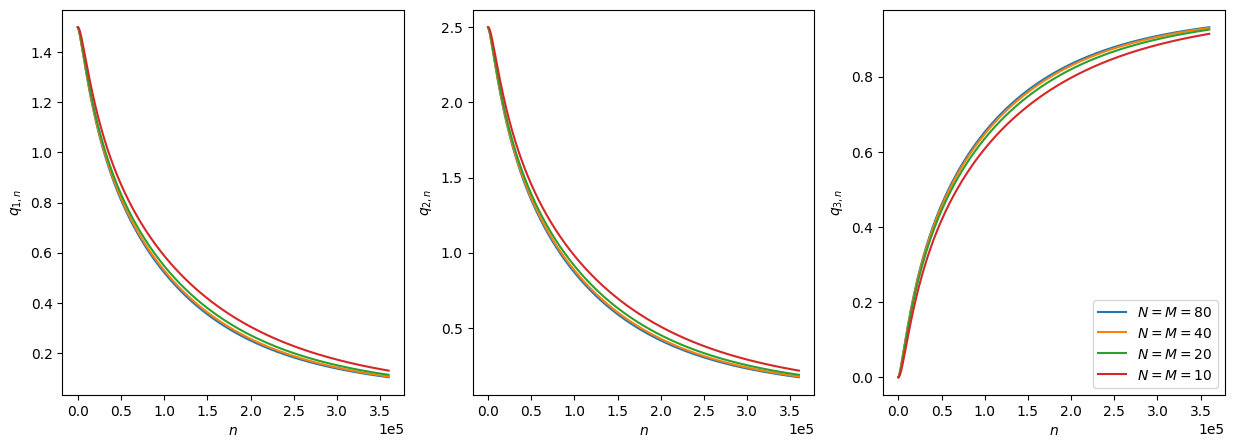
\includegraphics[width=\textwidth]{../assets/space-error-v2.png} \\
    \caption{Medžiagų priklausomybė nuo laiko. Čia $\tau=3.6\times 10^5$, $D=0.05$, $W = 1$, $H=1$, $k = 1$, $c_0 = 1$, $\Delta t = 1\times 10^{-5}$, $\Delta x$, $\Delta y$ - kintami ir priklauso nuo $N$ bei $M$ }
    %\label{result-example}
\end{figure}

Iš grafiko galima matyti, kad eksponentiškai didinant diskrečių taškų skaičių sprendinių grafikai duoda vis tikslesnius rezultatus. Taip pat galima pastebėti, kad kažkuriuo momentu diskrečios erdvės taškų didinimas nebeduoda ypatingai didelių rezultato pagerėjimų, taip yra todėl, išreikštinių skirtumų metodo paklaida yra antros eilės pagal erdvinius žingsnius $\Delta x$ ir $\Delta y$

\begin{align}
    \frac{\partial^2c}{\partial x^2}\Big|_{x=x_i, y=y_j, t=t_n}=\frac{c^n_{i-1,j} - 2c^n_{i,j} + c^n_{i+1,j}}{\Delta x^2} + \mathcal{O}(\Delta x^2)\\
    \frac{\partial^2c}{\partial y^2}\Big|_{x=x_i, y=y_j, t=t_n}=\frac{c^n_{i,j-1} - 2c^n_{i,j} + c^n_{i,j+1}}{\Delta y^2} + \mathcal{O}(\Delta y^2)
\end{align}

\subsection{Palyginimas su eksperimentiniais duomenimis}
